%$Header: /home/dashley/cvsrep/e3ft_gpl01/e3ft_gpl01/dtaipubs/cron/2006/wvecprob/wvecprob.tex,v 1.4 2006/12/26 06:59:37 dashley Exp $
%
\documentclass[letterpaper,10pt,titlepage]{article}
%
%\pagestyle{headings}
%
\usepackage{amsmath}
\usepackage{amsfonts}
\usepackage{amssymb}
\usepackage[ansinew]{inputenc}
\usepackage[OT1]{fontenc}
\usepackage{graphicx}
%\usepackage{makeidx}
%
%
%Define certain conspicuous global constants.
%\newcommand{\productbasename}{FBO-Prime}
%\newcommand{\productversion}{0.1}
%\newcommand{\productname}{\productbasename{}-\productversion}
%
%New environments
%The following environment is for the glossary of terms at the end.
%\newenvironment{docglossaryenum}{\begin{list}
%               {}{\setlength{\labelwidth}{0mm}
%                  \setlength{\leftmargin}{4mm}
%                  \setlength{\itemindent}{-4mm}
%                  \setlength{\parsep}{0.85mm}}}
%               {\end{list}}
%%
%The following environment is for the database table and field
%documentation at the end.
%\newenvironment{docdbtblfielddef}{\begin{list}
%               {}{\setlength{\labelwidth}{0mm}
%                  \setlength{\leftmargin}{10mm}
%                  \setlength{\itemindent}{-5mm}
%                  \setlength{\parsep}{0.85mm}}}
%               {\end{list}}
%%

%Embarrassingly, I've forgotten why "makeindex" is necessary ...
%\makeindex
%
\begin{document}
\title{A Least-Squares Solution to the Multiple-Aircraft Wind Estimation Problem}
\author{\vspace{1cm}\\David T. Ashley\\\texttt{dta@e3ft.com}\\\vspace{1cm}}
\date{\vspace*{8mm}\small{Version Control $ $Revision: 1.4 $ $ \\
      Version Control $ $Date: 2006/12/26 06:59:37 $ $ (UTC) \\
      $ $RCSfile: wvecprob.tex,v $ $ \\
      \LaTeX{} Compilation Date: \today{}}}
\maketitle

%%%%%%%%%%%%%%%%%%%%%%%%%%%%%%%%%%%%%%%%%%%%%%%%%%%%%%%%%%%%%%%%%%%%%%%%%%%%%%%
%
\begin{abstract}
This document presents a solution to the problem of estimating
wind speed and direction from simultaneous radar observations of the
course and groundspeed of multiple aircraft and knowledge of the approximate
cruising airspeed of each aircraft.

The problem was posted to the \texttt{sci.math} newsgroup by
Chad Speer in December, 2006.
\end{abstract}

%%%%%%%%%%%%%%%%%%%%%%%%%%%%%%%%%%%%%%%%%%%%%%%%%%%%%%%%%%%%%%%%%%%%%%%%%%%%%%%

\section{Introduction and Overview}
\label{siov0}

This problem was posted by Chad Speer to the \texttt{sci.math} newsgroup
in December, 2006\@.  The problem did not at that time receive any meaningful
suggestions toward a solution.

The problem is how to [uniquely] estimate wind velocity and direction
in the local area from:

\begin{itemize}
\item Radar observations of the course and groundspeed of multiple aircraft.
\item Knowledge of the cruising airspeed of each aircraft (typically obtained from
      VFR or IFR flightplan or clearance data filed by the pilot, or from knowledge
      of the model of aircraft).
\end{itemize}

This solution assumes that each observed aircraft is affected by wind at the
same speed and in the same direction.  This is a reasonable assumption, 
and will generally
hold true for aircraft at the same altitude separated by perhaps 
20-200 nautical miles.  However, this assumption may be very flawed
for aircraft at different altitudes, as the winds tend to vary greatly
in magnitude and direction with altitude.
(Relaxing the assumption of identical wind vectors affecting all observed aircraft
may be a direction for future mathematical refinement.)

Any mathematical results shown to work well in practice may eventually be
incorporated into algorithms used in air traffic control radar.

%%%%%%%%%%%%%%%%%%%%%%%%%%%%%%%%%%%%%%%%%%%%%%%%%%%%%%%%%%%%%%%%%%%%%%%%%%%%%%%

\section{Terms and Mathematical Nomenclature}
\label{snom0}

All angular measurements (the angles of vectors) are in degrees clockwise from true
North, and are expressed canonically where possible so that
$0^\circ \leq \theta < 360^\circ$.   $0^\circ$ is true North, $90^\circ$ is true East, 
$180^\circ$ is true South, and $270^\circ$ is true West.

The \emph{heading} of an aircraft is the direction the aircraft is pointed, whereas the
\emph{course} is the direction of the ground path of the aircraft.  In the presence
of wind other than a direct headwind or tailwind, the heading is unequal to the course.
The heading of the aircraft is known by the pilot but not reported to anyone on the ground.
The course of the aircraft is known from radar data.

Vectors are differentiated from scalars with an overlying arrow---$v_i$ is a scalar
but $\vec{v_i}$ is a vector. 

The local wind vector is $\vec{w}$ with magnitude $v_w$ and direction
$\theta_w$.

Each aircraft is denoted $A_i$, $i \in \{1, 2, \ldots{} \}$; and has a heading vector
$\vec{v_{hAi}}$ with magnitude $v_{hAi}$ and heading direction $\theta_{hAi}$.
The course of the aircraft $A_i$ is denoted as a vector $\vec{v_{cAi}}$ with magnitude
$v_{cAi}$ and course direction $\theta_{cAi}$.  Note that the course is observed by radar.

%%%%%%%%%%%%%%%%%%%%%%%%%%%%%%%%%%%%%%%%%%%%%%%%%%%%%%%%%%%%%%%%%%%%%%%%%%%%%%%

\section{The Wind Triangle}
\label{swtr0}

Airplanes fly in a moving block of air, so that the aircraft's ground motion is the
vector sum of the air motion with respect to the ground and the aircraft's
motion with respect to the air (Fig. \ref{fig:swtr0:00}).

For each aircraft $A_i$,

\begin{equation}
\label{eq:swtr0:01}
\vec{v_{cAi}} = \vec{w} + \vec{v_{hAi}} .
\end{equation}

(\ref{eq:swtr0:01}) is known as the \emph{wind triangle} because student pilots
are taught to make this calculation graphically by drawing a triangle of 
three vectors on graph paper or by using a mechanical computer such as the
E-6B\footnote{\texttt{http://en.wikipedia.org/wiki/E6B}.}.

\begin{figure}
\centering
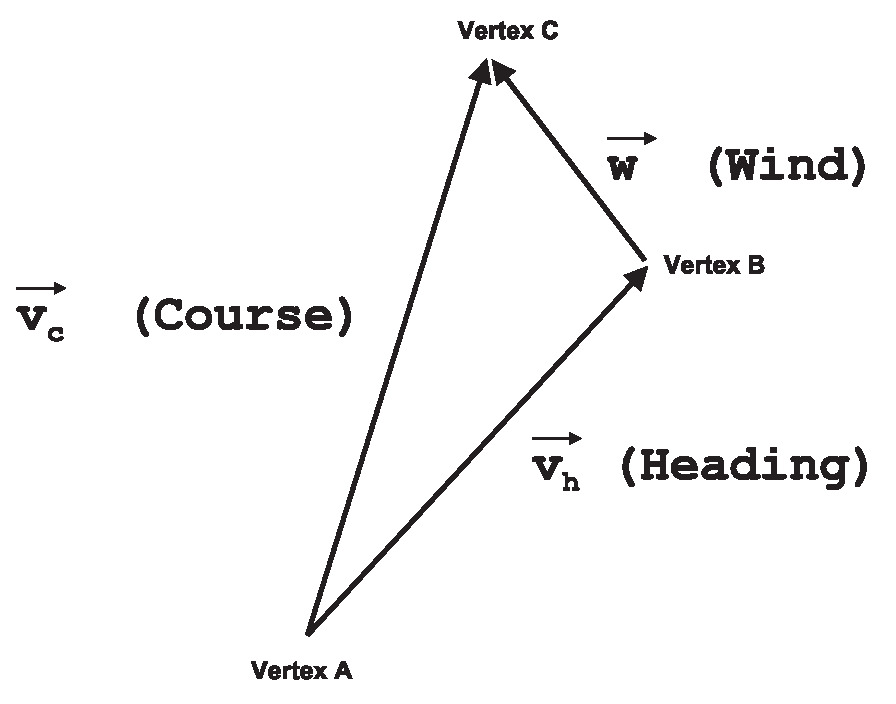
\includegraphics[height=3.0in]{wtri01.eps}
\caption{Wind Triangle}
\label{fig:swtr0:00}
\end{figure}

To a person who has never piloted an aircraft, (\ref{eq:swtr0:01})
may be unexpected.  It is very common for pilots to have a course that
differs from the heading by more than 10 degrees; and this is
visually apparent in an airplane when tracking roads or freeways below or when
landing in a crosswind.


%%%%%%%%%%%%%%%%%%%%%%%%%%%%%%%%%%%%%%%%%%%%%%%%%%%%%%%%%%%%%%%%%%%%%%%%%%%%%%%

\section{The One-Aircraft Case}
\label{ssac0}

%%%%%%%%%%%%%%%%%%%%%%%%%%%%%%%%%%%%%%%%%%%%%%%%%%%%%%%%%%%%%%%%%%%%%%%%%%%%%%%

\subsection{Graphical Solution}
\label{ssac0:sgsl0}

With only a single aircraft $A_1$,

\begin{equation}
\label{eq:ssac0:sgls0:01}
\vec{v_{cA1}} = \vec{w} + \vec{v_{hA1}} .
\end{equation}

\noindent{}Separating (\ref{eq:ssac0:sgls0:01}) into x- and y-components yields

\begin{eqnarray}
\label{eq:ssac0:sgls0:02}
v_{cA1} \cos \theta_{cA1} & = & w \cos \theta_w + v_{hA1} \cos \theta_{hA1} \\
\label{eq:ssac0:sgls0:03}
v_{cA1} \sin \theta_{cA1} & = & w \sin \theta_w + v_{hA1} \sin \theta_{hA1}
\end{eqnarray}

\noindent{}The following quantities are known:

\begin{itemize}
\item $v_{cA1}$ (from radar observation of the aircraft).
\item $\theta_{cA1}$ (from radar observation of the aircraft).
\item $v_{hA1}$ (the cruising speed of the aircraft, usually 
                filed by the pilot as part of the VFR or IFR clearance process).
\end{itemize}

\noindent{}The following quantities are unknown:

\begin{itemize}
\item $w$ (wind velocity).
\item $\theta_{w}$ (wind direction).
\item $\theta_{hA1}$ (Note as discussed above that \emph{heading} and 
      \emph{course} are distinct.  The course is known from radar observation,
      but the heading---the direction the aircraft is pointed---is not 
      known.\footnote{More precisely, the heading is not known by anyone \emph{on
      the ground}.  The heading is indicated by at least one aircraft instrument
      and known to the pilot, but this information is not communicated to anyone
      else.})
\end{itemize}

With two equations and three unknowns, it would normally be expected that the solution is a
set that can be parameterized with one parameter.

\begin{figure}
\centering
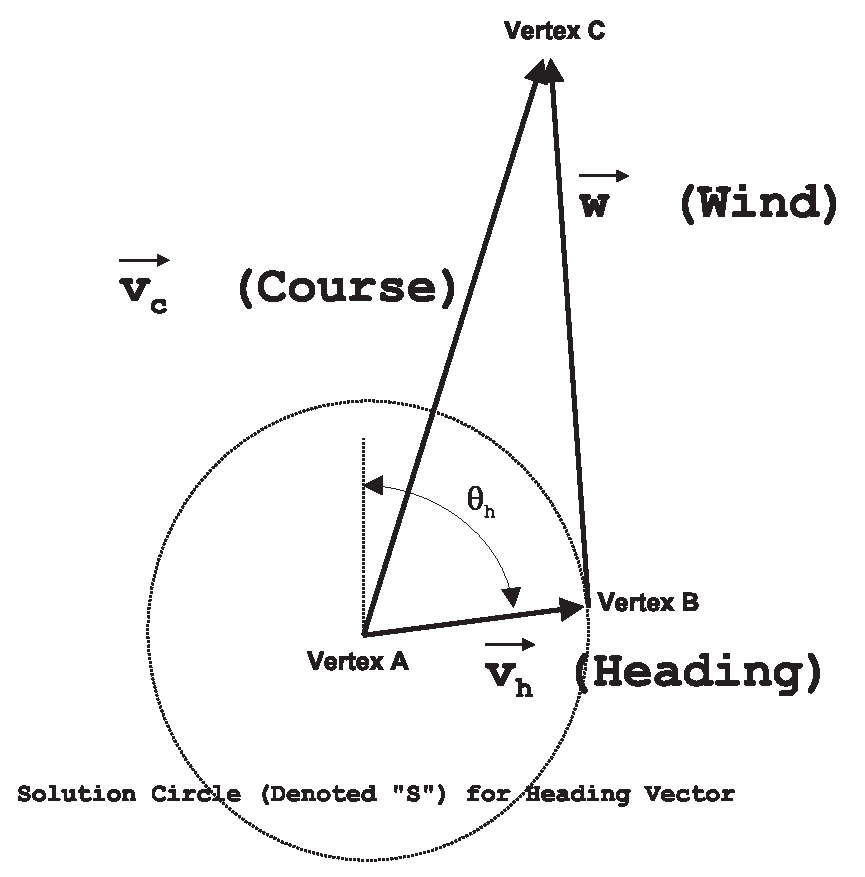
\includegraphics[width=4.0in]{ac1gsl01.eps}
\caption{Graphical Solution for One-Aircraft Case}
\label{fig:ssac0:sgls0:00}
\end{figure}
  
It can be seen graphically (Fig. \ref{fig:ssac0:sgls0:00}\footnote{Note that
although Fig. \ref{fig:ssac0:sgls0:00} conveys all the essential features of
the one-aircraft case, the wind vector $\vec{w}$ normally has the smallest magnitude
of the three vectors in the wind triangle.  A light aircraft that cruises
at 120 knots airspeed and is affected by winds of 10-30 knots is the typical case.}) 
that an infinite number of solutions
exist, parameterized by $0^\circ \leq \theta_{hA1} < 360^\circ$.  
A heading vector with the appropriate magnitude
($v_{hA1}$, the cruising speed of the aircraft) can be chosen so that its endpoint is
anywhere on the circle $C$ in Fig. \ref{fig:ssac0:sgls0:00}, and a wind vector $\vec{w}$
can then be chosen to solve the equations.

%%%%%%%%%%%%%%%%%%%%%%%%%%%%%%%%%%%%%%%%%%%%%%%%%%%%%%%%%%%%%%%%%%%%%%%%%%%%%%%

\subsection{Analytic Solution}
\label{ssac0:sasl0}

The problem can be solved analytically as follows:

\begin{itemize}
\item Choose $\theta_{hA1} \in [0^\circ, 360^\circ)$.
\item Since $\theta_{hA1}$ and $v_{hA1}$ are established,
      $\vec{v_{hA1}}$ is established.
      Solve for $\vec{w}$ using (\ref{eq:ssac0:sgls0:01}):

      \begin{equation}
      \label{eq:ssac0:sasl0:01}
      \vec{w} = \vec{v_{cA1}} - \vec{v_{hA1}}   .
      \end{equation}

\end{itemize}

%%%%%%%%%%%%%%%%%%%%%%%%%%%%%%%%%%%%%%%%%%%%%%%%%%%%%%%%%%%%%%%%%%%%%%%%%%%%%%%

\section{The Two-Aircraft Case}
\label{stac0}

%%%%%%%%%%%%%%%%%%%%%%%%%%%%%%%%%%%%%%%%%%%%%%%%%%%%%%%%%%%%%%%%%%%%%%%%%%%%%%%

\subsection{Graphical Solution}
\label{stac0:sgls0}

\begin{figure}
\centering
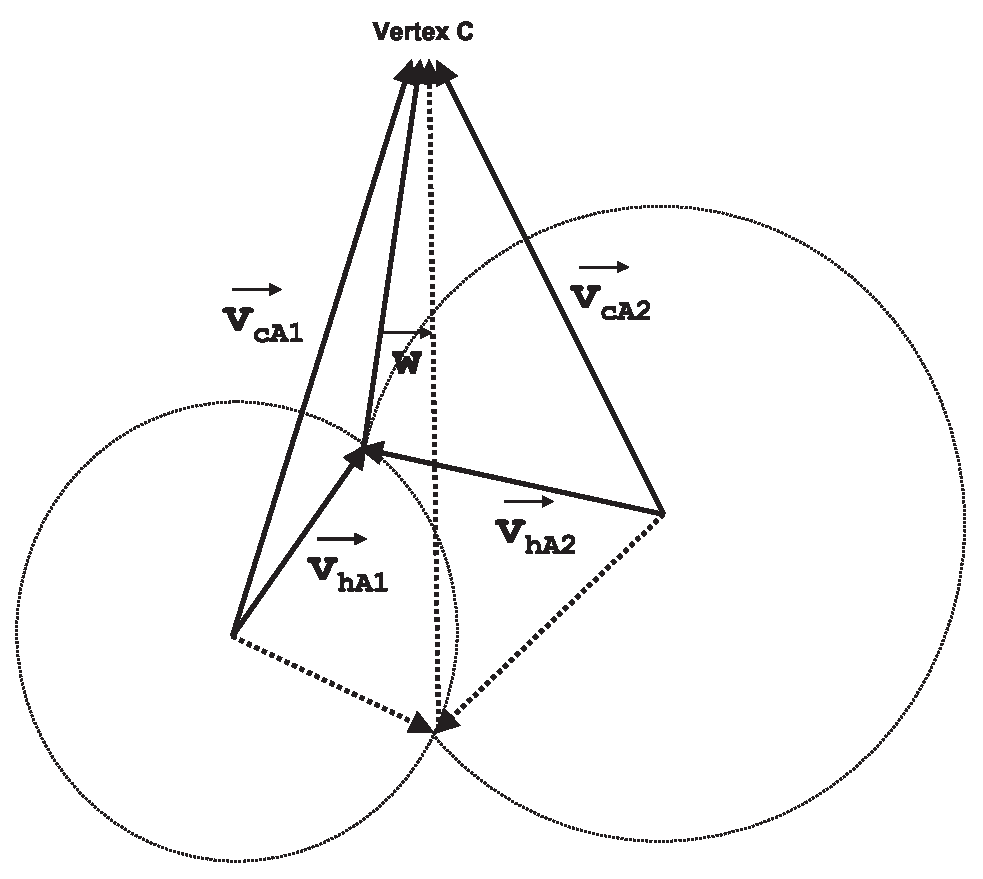
\includegraphics[width=4.0in]{ac2gsl01.eps}
\caption{Graphical Solution for Two-Aircraft Case}
\label{fig:stac0:sgls0:00}
\end{figure}

The two-aircraft case can be solved graphically by constructing the
solution sets (circle \emph{S} in Fig. \ref{fig:ssac0:sgls0:00}) 
of the two aircraft so that \emph{Vertex C}
(Figs. \ref{fig:swtr0:00}, \ref{fig:ssac0:sgls0:00}) are coincident.
Figure \ref{fig:stac0:sgls0:00} depicts the graphical solution.

Figure \ref{fig:stac0:sgls0:00} depicts the case where 
$A_2$ has a higher cruising speed (a solution circle of larger
radius) than $A_1$.  The following properties can be
observed from Fig. \ref{fig:stac0:sgls0:00}:

\begin{itemize}
\item Since the solution set for each aircraft is represented by a circle,
      the solutions for the two-aircraft case are the points where the two
      circles meet.
\item There may be no solutions, one solution, or two solutions for the
      two-aircraft case.  (Fig. \ref{fig:stac0:sgls0:00}
      depicts the case with two solutions.  The second solution is shown
      with dotted lines.)
\item In a practical case, the correct solution would probably be the
      solution with the wind vector of lesser magnitude.
\end{itemize}

%%%%%%%%%%%%%%%%%%%%%%%%%%%%%%%%%%%%%%%%%%%%%%%%%%%%%%%%%%%%%%%%%%%%%%%%%%%%%%%

\subsection{Analytic Solution}
\label{stac0:sasl0}

I have not a clue how to think about this problem analytically.

%%%%%%%%%%%%%%%%%%%%%%%%%%%%%%%%%%%%%%%%%%%%%%%%%%%%%%%%%%%%%%%%%%%%%%%%%%%%%%%

\section{The General Multiple Aircraft Case}
\label{smac0}

It is unclear how to set this up as a problem so that a unique solution
can be obtained in the presence of [mildly] inconsistent data, or what the basis
for the unique solution should be (i.e. similar to least-squares---there has
to be something one is trying to optimize or minimize).


%%%%%%%%%%%%%%%%%%%%%%%%%%%%%%%%%%%%%%%%%%%%%%%%%%%%%%%%%%%%%%%%%%%%%%%%%%%%%%%
\end{document}
%%%%%%%%%%%%%%%%%%%%%%%%%%%%%%%%%%%%%%%%%%%%%%%%%%%%%%%%%%%%%%%%%%%%%%%%%%%%%%%
% $Log: wvecprob.tex,v $
% Revision 1.4  2006/12/26 06:59:37  dashley
% Edits.
%
% Revision 1.3  2006/12/23 21:10:01  dashley
% Edits.
%
% Revision 1.2  2006/12/23 20:27:11  dashley
% Edits.
%
% Revision 1.1  2006/12/23 19:06:00  dashley
% Initial checkin.
%%%%%%%%%%%%%%%%%%%%%%%%%%%%%%%%%%%%%%%%%%%%%%%%%%%%%%%%%%%%%%%%%%%%%%%%%%%%%%%
